\documentclass[letterpaper]{article}
\usepackage[T1]{fontenc}
\usepackage{spconf,amsmath,graphicx,booktabs}
\usepackage{newtxmath}
\usepackage[hidelinks]{hyperref}

\urlstyle{same}
\hypersetup{pdftitle={Validation Speaker Exposure and Checkpoint Selection in Speech Emotion Recognition},pdfauthor={Tian Xie}}
\title{Validation Speaker Exposure and Checkpoint Selection\\in Speech Emotion Recognition}
\name{Tian Xie}
\address{University of Toronto\\tianjack.xie@mail.utoronto.ca}
\begin{document}
\maketitle
\begin{abstract}
Validation speaker separation and checkpoint selection are often discussed together, although validation optimism and common-test performance are different quantities. We compare seen- and unseen-speaker validation using cross-entropy (CE) or unweighted average recall (UAR) along identical WavLM training trajectories. A frozen protocol covers 360 main trajectories and 24 controls across three native emotion-recognition tasks. With CE selection, seen-speaker validation yields higher common-test UAR by 0.935 percentage points on CREMA-D and 2.247 on SUBESCO; the corresponding CE-versus-UAR interactions are 0.937 and 2.560 points. These four contrasts survive six-test Holm correction. RAVDESS estimates remain uncertain. Descriptive seen-minus-unseen differences under UAR selection are close to zero, without establishing equivalence. Complete 15-epoch curves and whole-group controls constrain mechanistic interpretations. The results support criterion-dependent selection effects under this fixed program, rather than a universal advantage of speaker-independent validation.
\end{abstract}
\begin{keywords}
speech emotion recognition, speaker independence, checkpoint selection, validation, evaluation
\end{keywords}
\section{Introduction}
Speech emotion recognition (SER) is often evaluated on speakers not used for training. Speaker separation is an established evaluation concern. SERAB and Antoniou et al. explicitly separate training, validation and test speakers~\cite{serab,antoniou}. More generally, optimizing a finite-sample selection criterion can affect subsequent performance evaluation~\cite{cawley}. However, a validation score difference and a difference in the selected models' performance on an identical unfamiliar-speaker test are distinct quantities. A larger validation--test gap alone does not establish that the corresponding selection rule produces a worse test model.

Prior SER studies already compare random and actor-independent evaluation across datasets, models or repeated runs~\cite{ibrahim,zielonka,kumari}; matching training counts across speaker/text conditions also has precedent~\cite{atmaja}. Such comparisons establish the relevance of evaluation protocols, but may change training or test membership along with the boundary of interest. We therefore study a specified checkpoint-selection comparison: validation on familiar versus unfamiliar speakers, each using either cross-entropy or unweighted average recall (UAR), along one shared training trajectory and on one shared speaker-exclusive outer test. Holding the candidate trajectory fixed removes differences between training runs from this within-trajectory comparison. The validation groups still contain different people, so the contrast concerns the complete selection policies rather than an isolated voiceprint mechanism.

This design follows earlier analyses of corpora already used in this project~\cite{artifact}. It fixes one model configuration, all 15 candidate epochs and the analysis before the new fits. The principal quantities are the common-test difference between the two cross-entropy policies and its interaction with the choice of cross-entropy versus UAR. All three native corpus tasks and all six planned tests are retained. Full trajectories and a fixed-last-epoch training-group exchange provide descriptive context; they do not supply additional hypothesis tests or determine which results are reported.


\section{Experimental design}
\subsection{Shared-trajectory checkpoint-selection protocol}
\label{sec:final-program-methods}

The protocol specifies 360 main trajectories: 24 draws and five outer folds
per corpus, plus 24 paired CREMA-D control fits. Checkpoint rules share a
training trajectory and speaker-independent outer test set. CREMA-D,
SUBESCO, and RAVDESS retain six, seven, and eight native classes and
91, 20, and 24 speakers, respectively~\cite{cremad,subesco,ravdess}.
These corpora have prior research exposure. The protocol uses a private
pre-execution source/plan freeze, not public preregistration. New draws do
not create previously untouched data.

Within each draw, metadata hashing partitions speakers into five outer
folds, stratified by recorded sex; each speaker enters exactly one outer
fold. Outside each fold, disjoint development
groups A and B are sex-balanced and complete across chosen texts and
native classes. All query groups share texts disjoint from fit texts
(Table~\ref{tab:final-program-panels}); unused speakers remain excluded.
Frozen representatives are MD-preferred/otherwise XX for CREMA-D, T1 for
SUBESCO, and normal-intensity R1 for RAVDESS, without substitute takes.
Outer queries retain available representatives, requiring all native
classes for every outer speaker. Insufficient development capacity causes
metadata failure, not outcome-dependent resampling.

\begin{table}[t]
\centering
\caption{Prespecified per-context allocation. A and B are equal-sized,
sex-balanced groups; counts denote distinct speakers or recordings.}
\label{tab:final-program-panels}
\small
\setlength{\tabcolsep}{3pt}
\begin{tabular}{lrrrcrr}
\hline
Corpus & Classes & A/B & Outer & Texts$^a$ & Fit & Query$^b$\\
\hline
CREMA-D & 6 & 24/24 & 17/19 & 4/2 & 576 & 288\\
SUBESCO & 7 & 8/8 & 4 & 4/2 & 224 & 112\\
RAVDESS & 8 & 8/8 & 4/6 & 1/1 & 64 & 64\\
\hline
\end{tabular}
\par\raggedright\small
$^a$ Fit/query text counts. $^b$ Recordings in each of A and B query;
outer queries contain available CREMA-D representatives, 56 SUBESCO
recordings, or 32/48 RAVDESS recordings. Slash-separated outer counts
denote alternative fold sizes.
\end{table}

Main trajectories train on A. WavLM base-plus~\cite{wavlm} has a
native-class linear head over mean-pooled final features; only the top
four Transformer layers and head are trainable. The earlier study's fixed
cfg3 uses AdamW,
encoder/head learning rates $5\times10^{-5}/10^{-3}$, weight decay 0.01,
batch size 16, and unweighted cross-entropy. All 15 epochs traverse the
fit set, without early stopping or hyperparameter search. Training uses
FP16 autocast with FP32 parameters; evaluation uses FP32.
Mono 16\,kHz audio is silence-trimmed at 30\,dB; training uses three-second crops
or zero-padding, and evaluation retains at most the first ten seconds.

A queries provide seen-speaker validation; B queries provide unseen-speaker
validation. All 15 epochs record A, B, and outer logits. Four rules minimize
mean cross-entropy or maximize UAR on A or B; exact ties select the earliest
epoch, using rational recall to preserve exact UAR ties.
UAR is macro recall over native classes in the whole query group,
not average speaker UAR. Each group has separate sorted batches of 16,
fixed across epochs and paired models. Outer audio cannot pad validation
batches. Pooling lacks a length mask: padding context is fixed, but padding
effects remain.

\begin{table*}[t]
\centering\small
\caption{The six prespecified common-test effects in UAR pp, pointwise 95\% draw-level $t$ intervals, and two-sided raw and six-family Holm $p$ values.}
\label{tab:primary}
\setlength{\tabcolsep}{5pt}
\begin{tabular}{llrrrr}\toprule
Corpus & Contrast & Mean & Pointwise 95\% CI & Raw $p$ & Holm $p$\\\midrule
CREMA-D & $\delta_{\mathrm{CE}}$ & 0.935 & [0.287, 1.583] & 0.0066 & 0.0264\\
CREMA-D & $J$ & 0.937 & [0.210, 1.663] & 0.0138 & 0.0413\\
SUBESCO & $\delta_{\mathrm{CE}}$ & 2.247 & [0.945, 3.549] & 0.0016 & 0.0083\\
SUBESCO & $J$ & 2.560 & [1.103, 4.016] & 0.0014 & 0.0083\\
RAVDESS & $\delta_{\mathrm{CE}}$ & 0.486 & [-0.198, 1.170] & 0.1549 & 0.3098\\
RAVDESS & $J$ & 0.469 & [-0.633, 1.570] & 0.3877 & 0.3877\\\bottomrule
\end{tabular}
\end{table*}

\begin{table*}[t]
\centering\small
\caption{Descriptive outer UAR (\%) of the four checkpoint policies and fixed epoch 15, plus $\delta_{\mathrm{UAR}}$ in pp; five folds then 24 draws are equally weighted.}
\label{tab:absolute}
\setlength{\tabcolsep}{5pt}
\begin{tabular}{lrrrrrr}\toprule
Corpus & Seen CE & Unseen CE & Seen UAR & Unseen UAR & Last 15 & $\delta_{\mathrm{UAR}}$\\\midrule
CREMA-D & 56.253 & 55.318 & 57.154 & 57.155 & 53.715 & -0.002\\
SUBESCO & 47.113 & 44.866 & 47.426 & 47.738 & 47.292 & -0.313\\
RAVDESS & 33.941 & 33.455 & 32.943 & 32.925 & 32.821 & 0.017\\\bottomrule
\end{tabular}
\end{table*}

Let $T(g,q)$ be outer UAR in percent at the epoch selected by group
$g$ (seen $s$, unseen $u$) and criterion $q$. Per-context contrasts are
\begin{align}
\delta_q &= T(s,q)-T(u,q),\quad q\in\{\mathrm{CE},\mathrm{UAR}\},\\
J &= \delta_{\mathrm{CE}}-\delta_{\mathrm{UAR}}.
\end{align}
These are outer UAR differences in percentage points (pp), not loss or
validation-optimism ($V-T$) differences. They compare selection rules,
without identifying a unique speaker mechanism. Four rules reuse one
trajectory; they do not require four training runs.

Within each corpus, five fold effects are averaged equally per draw.
Two-sided one-sample $t$ inference uses 24 complete draw effects ($df=23$).
The six-test family comprises $(\delta_{\mathrm{CE}},J)$ in three corpora,
with Holm control at 0.05 and pointwise 95\% $t$ intervals.
Undefined zero-variance tests remain NA, retaining their family slots.
Absolute UAR and $\delta_{\mathrm{UAR}}$ are descriptive. The 1\,pp practical
reference is not an equivalence margin; no equivalence test is performed.
Inference conditions on the finite corpus and training program; folds,
recordings, repeated speakers, and rules are not extra replicates.
Different native tasks preclude pooled inference or language-effect claims.

CREMA-D fold 0 adds one B-trained model per draw, sharing initial weights,
matched stochastic schedules, and sex/text/class fit-slot budgets with A.
Within each sex, slots also match speaker rank, take, and intensity.
B trains for 15 epochs and records only final queries, without checkpoint
selection. For whole-group query UAR $Q_A,Q_B$ in percent,
\begin{equation}
\begin{aligned}
E=\tfrac12\{&[Q_A(M_{A,15})-Q_A(M_{B,15})]\\
&+[Q_B(M_{B,15})-Q_B(M_{A,15})]\}.
\end{aligned}
\end{equation}
The 24 pairs and their mean are descriptive. This replaces whole training
groups, not individual speakers; these queries also select main-A
checkpoints.

\begin{figure*}[t]
\centering
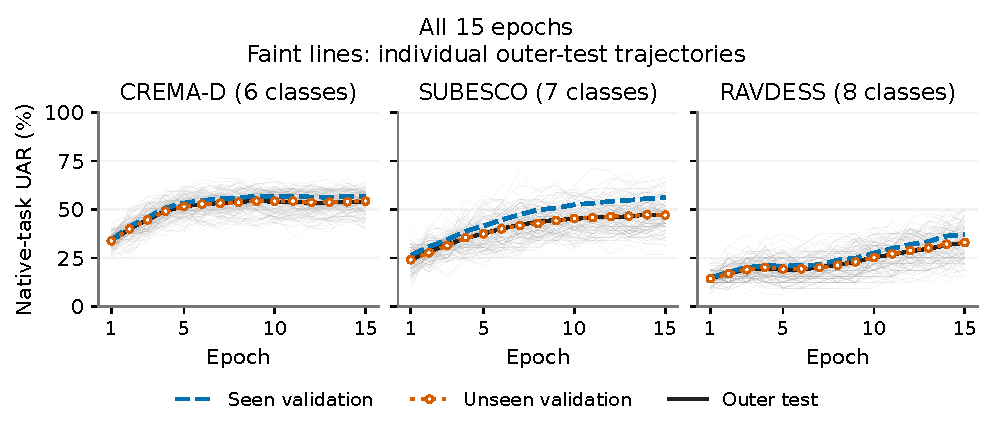
\includegraphics[width=178mm]{../figures/complete_epoch_curves.pdf}
\caption{All 15 epochs in the three native tasks. Faint grey lines are the 120 individual outer-test trajectories per corpus. The three heavy curves equally average the 120 main contexts for seen validation, unseen validation and outer testing. No smoothing or curve uncertainty bands are added.}
\label{fig:curves}
\end{figure*}

Four technical pilots are excluded from the 384 fits. Scoring requires
complete source, artifact, checkpoint, and ledger verification. Prespecified
descriptions retain selected-epoch distributions and agreement, all
15 epochs' outer curves, final UAR, epochs 8--10 minus 14--15 mean UAR,
and shortfall from each trajectory's maximum outer UAR. This oracle
neither selects retained checkpoints nor extends training. Full processing,
randomization, and verification details accompany the frozen protocol.

\section{Results}
\subsection{Prespecified common-test effects}
Table~\ref{tab:primary} reports the complete six-test family. Seen-CE selection exceeds unseen-CE selection by 0.935\,pp on CREMA-D and 2.247\,pp on SUBESCO; their pointwise intervals exclude zero and Holm-adjusted $p$ values are 0.0264 and 0.0083. Positive interactions of 0.937 and 2.560\,pp also survive Holm correction. Thus the seen--unseen selection contrast depends on the criterion in these two tasks. CREMA-D's CE estimate is below the 1\,pp reference; SUBESCO's exceeds it, but both intervals include 1\,pp. These tests do not establish effects larger than that reference.

RAVDESS gives $\delta_{\mathrm{CE}}=0.486$\,pp and $J=0.469$\,pp, with both intervals crossing zero. This is inconclusive evidence, not a third confirmed effect or equivalence. No corpus was dropped and no additional fits or tests were added after inspection.

\subsection{Absolute performance and selection behavior}
Table~\ref{tab:absolute} retains all four policies and epoch 15. Under UAR selection, the descriptive seen--unseen differences are $-0.002$, $-0.313$ and $+0.017$\,pp. Their small means do not establish equivalence. UAR-selected models have higher mean outer UAR than CE-selected models in CREMA-D and SUBESCO, whereas RAVDESS shows the opposite ordering. These within-task descriptive rankings do not support a universally best criterion.

Mean seen/unseen CE epochs are 6.71/5.89, 10.71/7.92 and 14.35/13.86 in corpus order; UAR means are 10.53/10.09, 12.54/11.98 and 13.66/13.48. CE epoch agreement is 58.3\%, 26.7\% and 76.7\%; UAR agreement is 37.5\%, 27.5\% and 42.5\%. Similar aggregate UAR contrasts therefore need not mean selection of the same epoch. Full distributions and oracle shortfalls accompany the artifact. On CREMA-D, the mean oracle shortfall is 2.34/3.27\,pp for seen/unseen CE, about 1.44\,pp for either UAR rule, and 4.88\,pp at epoch 15; these are descriptive shortfalls from trajectory-wise outer-test maxima, not attainable selection guarantees.

\subsection{Complete trajectories and whole-group exchange}
Figure~\ref{fig:curves} shows a CREMA-D plateau and continued mean outer improvement on SUBESCO and RAVDESS. The prespecified mean UAR at epochs 8--10 minus epochs 14--15 is $+0.208$, $-2.894$ and $-8.977$\,pp. The curves therefore do not support a uniform late-training collapse explanation. RAVDESS selects epoch 15 in 72/120 seen-CE and 62/120 unseen-CE trajectories; the fixed horizon limits interpretation of later behavior.

The CREMA-D training-group exchange has mean $E=2.828$\,pp across 24 pairs. All pair values, including the negative pair, are retained in the artifact. This is consistent with an average advantage on queries from the model's own training-speaker group under matched slots. It neither isolates individual speaker causality nor establishes why CE and UAR choose different checkpoints.

\section{Discussion}
The main finding is criterion-dependent common-test selection behavior. Speaker-exclusive validation remains an established way to evaluate generalization, but that rationale does not guarantee that its CE-selected checkpoint outperforms a seen-CE checkpoint on the same outer test. Conversely, these results do not justify replacing speaker-independent reporting with seen-speaker scores: model selection and reported evaluation answer different questions. CE measures probability quality whereas UAR depends on class decisions; their distinction offers a plausible explanation to investigate, not a tested calibration mechanism.

Earlier project studies~\cite{artifact} help separate the estimands. N14R2 found a 1.419\,pp difference in validation optimism, $\Delta(V-T)$, while inner procedures also changed fitting membership. DUAL held fitting trajectories common and found a 2.706\,pp optimism contrast while the selected outer-score difference was positive. These quantities are not the present $\delta_q$. Subsequent checkpoint diagnostics motivated this fixed-configuration study; they are post hoc uses of existing predictions, not independent replication. Shared corpora and previous fits do not enlarge the current inferential sample.

\subsection{Scope and data-construction implications}
The estimates condition on finite acted-speech corpora, one partially fine-tuned encoder, and the fixed training horizon. Tasks differ in native classes, speaker counts, texts and fit sizes; they identify neither a language effect nor a fair ranking of corpus difficulty. Validation identities and recording distributions also differ, precluding an isolated voiceprint interpretation. Fixed role batches preserve padding context without eliminating its effects. The group-exchange queries also participate in main-model selection and are not globally unused blind tests.

Related data-construction studies answer narrower questions. At fixed recording counts, increasing speakers also reduced text coverage per speaker; CNN gains of 1.08/2.16\,pp on unseen texts at 288/576 recordings, respectively, estimate that joint tradeoff. A separate voiceprint-coverage policy gave CNN $-0.109$\,pp relative to uniform selection (conditional paired-person bootstrap 95\% interval $[-0.715,0.509]$), without establishing equivalence or general futility of coverage. These studies and their full results remain in the artifact, rather than a pooled confirmation of the present endpoint. Synthetic-speech training was not admitted: technical generation and incomplete human evaluation did not satisfy the quality protocol. A dataset that eliminates the seen--unseen gap has not been demonstrated.

\subsection{Execution and availability}
All 384 formal fits completed on one RTX 5070, with no training retries; four pilots were excluded. Unit wall times total 4.78 hours, including prescribed evaluation and saving. The artifact records 110,160 update attempts and 44 AMP skips. Full source/artifact/checkpoint/ledger verification and independent numerical replay passed. Fresh-process restoration of the four predetermined units reproduced 30 saved-state/query-group comparisons exactly, after correcting a documented launcher environment error. This limited check is not independent retraining. A portable prediction package passed numerical replay after extraction; it excludes audio, base weights and checkpoints. The artifact is access-restricted at preparation. Its private freeze establishes version history, not public preregistration.

\section{Conclusion}
On shared WavLM trajectories and outer tests, CE-based seen-speaker selection performed better on CREMA-D and SUBESCO, with evidence that the exposure contrast changes under UAR selection. RAVDESS remains uncertain, and full curves do not support uniform late-training collapse in these runs. The contribution is a controlled selection-policy comparison with criterion dependence, not a universal validation prescription or an identified speaker/language mechanism.

\section{Acknowledgments and AI disclosure}
Anthropic Claude assisted original implementation, drafting and scientific review. OpenAI Codex assisted experiment design, implementation/execution, literature and analysis verification, and drafting/revision of all manuscript sections and tables. These systems are not authors; the named human author is responsible for reviewing the evidence and approving submission. The experiments use existing datasets; no new participant data were collected.

\clearpage
\begin{thebibliography}{12}
\raggedright
\bibitem{serab} N. Scheidwasser-Clow, M. Kegler, P. Beckmann, and M. Cernak, ``SERAB: A multi-lingual benchmark for speech emotion recognition,'' in \emph{Proc. ICASSP}, 2022, pp. 7697--7701, doi: 10.1109/ICASSP43922.2022.9747348.
\bibitem{antoniou} N. Antoniou, A. Katsamanis, T. Giannakopoulos, and S. Narayanan, ``Designing and evaluating speech emotion recognition systems: A reality check case study with IEMOCAP,'' in \emph{Proc. ICASSP}, 2023, pp. 1--5, doi: 10.1109/ICASSP49357.2023.10096808.
\bibitem{cawley} G. C. Cawley and N. L. C. Talbot, ``On over-fitting in model selection and subsequent selection bias in performance evaluation,'' \emph{Journal of Machine Learning Research}, vol. 11, no. 70, pp. 2079--2107, 2010.
\bibitem{ibrahim} E. Ibrahim, M. E. Ghoraba, and A. E. Ghoraba, ``Multimodal emotion recognition using hybrid deep feature fusion under speaker-independent evaluation,'' \emph{Scientific Reports}, vol. 16, Art. 19584, 2026, doi: 10.1038/s41598-026-58836-w.
\bibitem{zielonka} M. Zielonka et al., ``Recognition of emotions in speech using convolutional neural networks on different datasets,'' \emph{Electronics}, vol. 11, no. 22, Art. 3831, 2022, doi: 10.3390/electronics11223831.
\bibitem{kumari} P. Kumari et al., ``Hybrid CNN-embedding fusion with MFCC-SVM for speech emotion recognition: Random vs actor-wise evaluation on CREMA-D,'' \emph{PLOS One}, vol. 21, no. 8, Art. e0355238, 2026, doi: 10.1371/journal.pone.0355238.
\bibitem{atmaja} B. T. Atmaja and A. Sasou, ``Effect of different splitting criteria on the performance of speech emotion recognition,'' in \emph{Proc. TENCON}, 2021, pp. 760--764, doi: 10.1109/TENCON54134.2021.9707265.
\bibitem{artifact} T. Xie, ``SER: Speaker-validation studies and the completed checkpoint-selection program,'' GitHub repository, 2026. [Online; access restricted at manuscript preparation]. \url{https://github.com/DeerNeverStop/SER}. Frozen scientific commit: \texttt{976297d}; completed evidence: \texttt{SER26-final-program-}\allowbreak\texttt{complete-20260907}. Earlier N14R2, DUAL, recording-budget and coverage results are retained with their separate protocols.
\bibitem{cremad} H. Cao, D. G. Cooper, M. K. Keutmann, R. C. Gur, A. Nenkova, and R. Verma, ``CREMA-D: Crowd-sourced emotional multimodal actors dataset,'' \emph{IEEE Trans. Affective Computing}, vol. 5, no. 4, pp. 377--390, 2014, doi: 10.1109/TAFFC.2014.2336244.
\bibitem{subesco} S. Sultana, M. S. Rahman, M. R. Selim, and M. Z. Iqbal, ``SUST Bangla Emotional Speech Corpus (SUBESCO): An audio-only emotional speech corpus for Bangla,'' \emph{PLOS ONE}, vol. 16, no. 4, Art. e0250173, 2021, doi: 10.1371/journal.pone.0250173.
\bibitem{ravdess} S. R. Livingstone and F. A. Russo, ``The Ryerson Audio-Visual Database of Emotional Speech and Song (RAVDESS): A dynamic, multimodal set of facial and vocal expressions in North American English,'' \emph{PLOS ONE}, vol. 13, no. 5, Art. e0196391, 2018, doi: 10.1371/journal.pone.0196391.
\bibitem{wavlm} S. Chen et al., ``WavLM: Large-scale self-supervised pre-training for full stack speech processing,'' \emph{IEEE J. Sel. Topics Signal Process.}, vol. 16, no. 6, pp. 1505--1518, 2022, doi: 10.1109/JSTSP.2022.3188113.
\end{thebibliography}
\end{document}
